\setcounter{chapter}{4}
\chapter{Meccanica Hamiltoniana}
\section{Introduzione}
La formulazione delle leggi della meccanica mediante la funzione Lagrangiana, descrive l'evoluzione di un sistema meccanico utilizzando le coordinate di posizione e velocit\'{a} generalizzate che incorporano l'informazione della forza esercitata dai vincoli senza doverne conoscere esplicitamente la forma. Per\`{o} non \`{e} l'unico modo in cui \`{e} possibile descrivere lo stato dinamico di un sistema. Infatti si pu\'{o} studiare un sistema rispetto alle coordinate di posizione e quantit\`{a} di moto generalizzate. La trattazione di problemi utilizzando tale sistema di coordinate costituisce le basi dell'ottica, meccanica quantistica e meccanica statistica. Per passare da un sistema di coordinate indipendenti ad un altro si usa la \textbf{trasformazione di Legendre} che permette di definire una nuova grandezza che descrive l'energia totale del sistema, definita \textbf{Hamiltoniana}. Quanto discusso in questo capitolo presupone che si considerino vincoli olonomi e potenziali dipendenti dalla posizione e/o velocit\'{a}.

\section{Formalismo Hamiltoniano}

Abbiamo visto che introducendo la funzione Lagrangiana $\mathcal{L}(\underline{q}(t),\underline{\dot q}(t),t)$ che descrive una curva nello spazio delle coordinate generalizzate. La minimizzazione del suo funzionale d'azione ci permette di definire le equazioni di Eulero-Lagrange

\begin{equation}
	\frac{d}{d t} \frac{\partial \mathcal{L}}{\partial \dot{q}_{i}}-\frac{\partial \mathcal{L}}{\partial q_i}=0 \quad \quad \text{i} = 1,...,n
\end{equation} 	
La grandezza
\begin{equation}
	p_i=\frac{\partial L}{\partial \dot{q}_i} \quad \quad \quad \text{i} = 1,...,n
\end{equation}
\`{e} definita \textbf{quantit\`{a} di moto generalizzata} coniugata a $q_i$ (e coincide con la quantit\`{a} di moto nelle coordinate cartesiane). Riscrivendo le equazioni di E-L con questa notazione si ha che la (5.1) diventa:
\begin{equation}
	\dot p_i = \frac{\partial L}{\partial \dot{q}_i}
\end{equation}
Lo scopo di riscrivere le equazioni in questo modo \`{e} di eliminare le velocit\`{a} generalizzate $\dot q_i$ in favore delle coordinate $p_i$. Il passaggio a $p_i$ ha un ruolo chiave perch\`{e} quando $p_i = 0$ si hanno delle coordinate cicliche, che come vedremo nei paragrafi successivi permettono di risolvere facilmente le equazioni differenziali che definiscono la dinamica del moto nello spazio delle fasi.
\subsubsection{Richiamo}
La quantit\`{a} $\{q_i \}$ definisce un punto nello \textit{spazio delle configurazioni C} di dimensione n. La sua evoluzione nel tempo definisce una curva in C. L'evoluzione dinamica del sistema \`{e} descritta dalle coordinate $\{q_i,p_i \}$ definite nello \textit{spazio delle fasi} di dimensione 2n. In tale spazio una cammino non incrocia mai con un altro e l'evoluzione \`{e} dunque governata da un \textit{flusso} che avviene nello spazio delle fasi.

 
\begin{figure}[ht]
\vspace{0.1in}
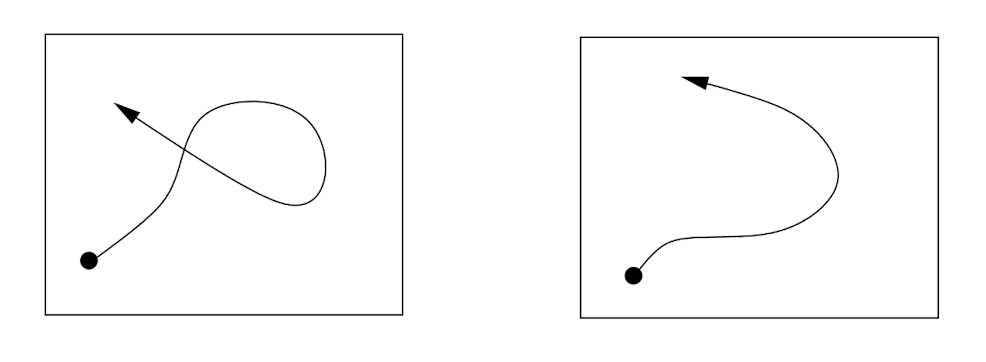
\includegraphics[scale = 0.5]{phase}	
\centering
\vspace{0.1in}
\caption{Moto nello spazio delle configurazioni (sinistra) e nello spazio delle fasi (destra)}
\end{figure}


\subsection{Equazioni di Hamilton}
Vogliamo determinare una funzione definita sullo spazio delle fasi che descriva in modo univoco l'evoluzione rispetto a $q_i$ e $p_i$. Questo vuol dire che deve essere in funzione di $q_i$ e $p_i$ e debba contenere la stessa informazione data dalla Lagrangiana $\mathcal{L}(\underline{q}(t),\underline{\dot q}(t),t)$. Per farlo utilizziamo una trasformazione di coordinate definita trasformazione di Legendre.
Definiamo la funzione \textbf{Hamiltoniana} come la trasformata di Legendre della Lagrangiana rispetto alle variabili $\dot q_i$.
\begin{equation}
	H\left(q_i, p_i, t\right)=\sum_{i=1}^n p_i \dot{q}_i-L\left(q_i, \dot{q}_i, t\right)
\end{equation}
Dove l'ipotesi fondamentale \`{e} data dal fatto che dalla relazione (5.2) sia possibile determinare $\dot q_i(q_i,p_i,t)$, ovvero si richiede che la trasformazione di coordinate sia invertibile rispetto alle $\dot q_i$.\newline
La variazione di H \`{e} data da:
\begin{equation}
	d H=\left(d p_i \dot{q}_i+p_i d \dot{q}_i\right)-\left(\frac{\partial L}{\partial q_i} d q_i+\frac{\partial L}{\partial \dot{q}_i} d \dot{q}_i+\frac{\partial L}{\partial t} d t\right)
\end{equation}
\begin{equation*}
	=d p_i \dot{q}_i-\frac{\partial L}{\partial q_i} d q_i-\frac{\partial L}{\partial t} d t
\end{equation*}
Il differenziale di sinistra pu\`{o} essere riscritto come
\begin{equation}
	d H=\frac{\partial H}{\partial q_i} d q_i+\frac{\partial H}{\partial p_i} d p_i+\frac{\partial H}{\partial t} d t
\end{equation}
l'uguaglianza ottenuta ci permetter di definire un sistema di equazione di 2n equazioni differenziali del primo ordine che prendono il nome di \textbf{equazioni di Hamilton}
\begin{align}
	\begin{cases}
	\dot{p}_i  =-\frac{\partial H}{\partial q_i} \\
	\dot{q}_i  =\frac{\partial H}{\partial p_i} \\
	\frac{\partial L}{\partial t} = -\frac{\partial H}{\partial t}
	\end{cases}	
\end{align}	
Rispetto alle equazioni di E-L che definivano un sistema di N equazioni differenziali del secondo ordine
abbiamo costruito un sistema di 2N equazioni differenziali del primo ordine.\newline
Si nota che la funzione di Hamilton coincide con l'energia del sistema E($q,\dot q, t$) data dall'\textbf{integrale di Jacobi} per la Lagrangiana di un sistema.

\subsection{Esempi}

\subsubsection{1) Particella in un potenziale}

Consideriamo una particella che si muove in un potenziale centrale in uno spazio a 3 dimensioni. La Lagrangiana sar\`{a} data da
\begin{equation*}
	L = \dfrac{1}{2}|\underline{\dot x}|^2 - U(\underline{x})
\end{equation*}
Le equazioni di E-L associate sono:
\begin{align}
	\begin{cases}
		\ddot x_1 = -\dfrac{dU(\underline{x})}{dx_1} \\
		\quad \;\,\vdots \\
		\ddot x_n = -\dfrac{dU(\underline{x})}{dx_n} 
	\end{cases}
	\quad \iff \quad
	\begin{cases}
		\dot x_1 = y_1 \\
		\dot y_1 = -\frac{dU(\underline{x})}{dx_i}\\
		\quad \;\,\vdots \\
		\dot x_n = y_n \\
		\dot y_n = - \frac{dU(\underline{x})}{dx_n}
	\end{cases}
\end{align}	
Usando la relazione (5.2) e (5.4) otteniamo
\begin{equation*}
	p=\frac{\partial \mathcal{L}}{\partial \dot{x}}=\dot{x} \quad \quad  \quad H=p \dot{x}-\mathcal{L}(x, \dot{x}(x, p))
\end{equation*}
dunque la Hamiltoniana associata al sistema \`{e} data da 
\begin{equation*}
H=p^2-\frac{p^2}{2}+U(x)=\frac{p^2}{2}+U(x)	
\end{equation*}
usando le equazioni in (5.7) definiamo le equazioni di Hamilton del sistema dinamico 
\begin{align*}
	\begin{cases}
		\dot x_i=p_i \\
		\dot p_i=-U^{\prime}(\underline{x})
	\end{cases}
	\quad i = 1,...,n
\end{align*}
posto $y_i = p_i$ nelle equazioni in (5.8) si ha che le equazioni di Hamilton e di E-L sono equivalenti tra loro.

\subsubsection{2) Invertibilit\`{a} delle velocit\`{a} generalizzate}

La Lagrangiana di un sistema \`{e} data da
\begin{equation*}
	\mathcal{L}=\frac{1}{2} g(q) \dot{q}^2-U(q)
\end{equation*}
dove g(q) \`{e} una funzione delle coordinate generalizzate e la quantit\`{a} di moto generalizzata \`{e} esprimibile come
\begin{equation*}
	p=g(q) \dot{q} \quad \text{dove} \quad g(q)>0 
\end{equation*}
di conseguenza la trasformazione di coordinate \`{e} invertibile, infatti
\begin{equation*}
	\dot q(q,p) = \dfrac{p}{g(q)}
\end{equation*}
e la Hamiltoniana associata al sistema pu\`{o} essere riscritta come
\begin{equation*}
	H = \dfrac{p^2}{2g(q)} + U(q)
\end{equation*}
dove le rispettive equazioni di Hamilton sono date da
\begin{align*}
	\begin{cases}
\frac{d u}{d t}=\frac{p}{g(q)} \\
 \frac{d}{d t} p=\frac{1}{2}\frac{g^{\prime}(q)}{g^2(q)} p^2-\frac{\partial}{\partial q} U \\
	\end{cases}
\end{align*}
\vspace{0.1in}

\begin{theorem}[Equivalenza Eq. E-L ed Hamilton ]
Le equazioni di Eulero-Lagrange sono equivalenti alle equazioni di Hamilton.
\end{theorem}

\begin{proof}
Partiamo da un Hamiltoniana definita rispetto ad un Lagrangiana indipendente dal tempo $\frac{\partial \mathcal{L}}{dt} = 0$ e consideriamo uno spazio delle configurazioni C in una sola dimensione. La variazione della funzione di Hamilton sar\`{a} descritta dal differenziale

\begin{equation*}
	d H(q, p, t)=\frac{\partial H}{\partial q} d q+\frac{\partial H}{\partial p} d p
\end{equation*}
\newline
ricordando che $\dot q (q,p,t)$ si ha che l'equazione precedente \`{e} equivalente a 
\begin{equation*}
	d(p \dot{q}-\mathcal{L}(q, \dot{q}, t))= pd\dot q +dp \dot q - \dfrac{\partial \mathcal{L}}{\partial q}dq - \dfrac{\partial \mathcal{L}}{\partial \dot q}d \dot q =
\end{equation*}
\begin{equation*}
	= pd\dot q +dp \dot q - \dfrac{\partial \mathcal{L}}{\partial q}dq - pd \dot q = \dot q dp - \dfrac{\partial \mathcal{L}}{\partial q}dq
\end{equation*}
\newline
dalle equazioni di E-L abbiamo che $\frac{d}{dt} \big [ \frac{\partial \mathcal{L}}{\partial \dot q} \big ] =\frac{\partial \mathcal{L}}{\partial  q} $ dunque l'uguaglianza precedente pu\`{o} essere riscritta come
\begin{equation*}
	=\dot q dp - \dfrac{d}{dt} \Big [\dfrac{\partial \mathcal{L}}{\partial \dot q} \Big ]dq = \dot q dp  + (- \dot p)dq
\end{equation*}
in conclusione otteniamo 
\begin{align*}
	\begin{cases}
	\dot{p}_i  =-\frac{\partial H}{\partial q_i} \\
	\dot{q}_i  =\frac{\partial H}{\partial p_i} \\
	\end{cases}
\end{align*}
\end{proof}

\begin{proof}
	Si consideri dim[C] $>1$ procediamo come nel caso in una dimensione definendo il differenziale dell'Hamiltoniana
\begin{equation*}
	d H=\sum_{j=1}^n \frac{\partial H}{\partial q_j} d q_j+\sum_{j=1}^n \frac{\partial H}{\partial p_j} d p_j+\frac{\partial H}{\partial t}
\end{equation*}
le j-sime equazioni possono essere riscritte come 
	\begin{alignat*}{2}
		\dfrac{\partial H}{\partial q_j}=\sum_i^n p_i \dfrac{\partial \dot{q}_i}{\partial q_j}-\dfrac{\partial \mathcal{L}}{\partial q_j}-\sum_{i=1}^n \dfrac{\partial \mathcal{L}}{\partial \dot{q}_j} \dfrac{\partial \dot{q}_i}{\partial q_j} = -\dfrac{\partial \mathcal{L}}{\partial q_j}+\underbrace{\sum_{i=1}^n \frac{\partial \dot{q}_i}{\partial q_j}\left[\frac{\partial \mathcal{L}}{\partial \dot{q}_i}-p_i\right]}_{=0} \\[0.05cm]
		\dfrac{\partial H}{\partial p_j}=\sum_i^n \dot{q}_i \dfrac{\partial p_i}{\partial p_j}+\sum_i^n p_i \dfrac{\partial \dot{q}_i}{\partial p_j}-\sum_i^n \dfrac{\partial \mathcal{L}}{\partial \dot{q}_i} \dfrac{\partial \dot{q}_i}{\partial p_j} = \dot{q}_j + \underbrace{\sum_i^n \frac{\partial \dot{q}_i}{\partial p_j}\left[\frac{\partial \mathcal{L}}{\partial \dot{q}_i}-p_i\right]}_{=0}\\[0.05cm]
		\dfrac{\partial H}{\partial t}=-\dfrac{\partial \mathcal{L}}{\partial t}-\sum_i^n \dfrac{\partial \mathcal{L}}{\partial \dot{q}_i} \dfrac{\partial \dot{q}_i}{\partial t}+\sum_i^n p_i \dfrac{\partial \dot{q}_i}{\partial t} = -\dfrac{\partial \mathcal{L}}{\partial t}+\underbrace{\sum_{i=1}^n \frac{\partial \dot{q}_i}{\partial t}\left[\dfrac{\partial \mathcal{L}}{\partial \dot{q}_i}-p_i\right]}_{=0}
	\end{alignat*}
di conseguenza si ottiene un sistema di 2N equazioni differenziali al primo ordine.
\end{proof}

\subsection{Leggi di conservazione}

\begin{lemma}
Se $\frac{\partial H}{\partial t} = 0$ allora H \`{e} una costante del moto
\end{lemma}

\begin{lemma}
	Se una coordinata trascurabile q non compare nella Lagrangiana allora per costruzione non apparte nemmeno nella Hamiltoniana. I momenti coniugati $p_q$ associati a q sono conservati.
\end{lemma}

\subsection{Momenti coniugati rispetto alla trasformazione di Legendre}

\begin{theorem}
Se la Lagrangiana di un sistema \`{e} rappresentabile come
\begin{equation}
	\mathcal{L} = \frac{1}{2} \sum_{\alpha, \beta}  G_{\alpha, \beta}  \cdot \dot{q}_\alpha \;\dot{q}_\beta-U = \frac{1}{2} \langle \underline{\dot q},G \underline{\dot q}\rangle - \;U
\end{equation}
dove G(q) \`{e} una matrice simmetrica ed invertibile associata all'energia cinetica del sistema $\Rightarrow$ si ha che il vettore dei momenti coniugati e le velocit\`{a} generalizzate possono essere scritte come
\begin{equation}
	\underline{p} = G(\underline{q})\cdot \underline{\dot q} \quad \text{e} \quad \dot q = G^{-1}(p) \cdot \underline p
\end{equation}
\end{theorem}

\subsubsection{Esempio}
La trasformata di Legendre definita da una Lagrangiana della forma come in (5.9) \'{e} data da
\begin{align*}
	 p \dot{q}=\frac{1}{2}\left\langle\dot{q}, G_{\dot{q}}\right\rangle+U &=\\
	&=\left\langle p, G^{-1} p\right\rangle-\frac{1}{2}\left\langle G^{-1} p, G G^{-1} p\right\rangle+U=\\
	&=\left\langle p, G^{-1} p\right\rangle-\frac{1}{2}\left\langle p, G^{-1} p\right\rangle+U
\end{align*}
dunque la Hamiltoniana associata \`{e} data da 
\begin{equation*}
	H = \dfrac{1}{2}\left\langle p, G^{-1} p\right\rangle + U
\end{equation*}

\begin{remark}
Data una matrice simmetrica invertibile, l'inversa \`{e} ancora una matrice simmetrica e $(G^{-1})^T = (G^T)^{-1}$.
\end{remark}

\subsection{Il principio di minima azione}

Consideriamo un punto $(q,\dot q) \in \Omega \subseteq \mathbb{R}^{2N}$ elemento dello spazio delle fasi, abbiamo che l'evoluzione della posizione del punto q nel tempo
\begin{equation}
	q : [t_0,t_1] \rightarrow \mathbb{R} \quad \text{t.c} \quad  q(t_0) = q_0 \quad \text{e} \quad q(t_1) = q_1
\end{equation}
definisce un cammino nello spazio delle configurazioni. Il numero di cammini che uniscono due punti nello spazio \`{e} infinito, dunque non \`{e} univoco, ci domandiamo quale sia il reale cammino che congiunge le due posizioni. Per rispondere a tale domanda introduzione una grandezza che \`{e} data dal funzionale d'azione.

\begin{equation}
	S: \mathcal{C}_{0,1} \rightarrow \mathbb{R} 	
\end{equation}
\begin{equation*}
	q \mapsto S[q] 
\end{equation*}
definita sullo spazio dei cammini, che \`{e} uno spazio affine modellato su uno spazio vettoriale di dimensione infinita. Dove 
\begin{equation}
	S\left[q(t)\right]=\int_{t_i}^{t_f} \mathcal{L}\left(q(t), \dot{q}(t)\right) d t
\end{equation}
e $\mathcal{L}$ definisce la Lagrangiana del sistema associata. L'azione  ha una propriet\`{a} significativa rispetto ai cammini di un sistema, ovvero il cammino effettivamente percorso dal sistema coincide con il suo estremo inferiore. 
\begin{lemma}
	Sia g(t) una funzione continua e derivabile in $[t_0,t_1]$ tale che $\forall \,h(t)$ continua in $[t_0,t_1]$ se 
	\begin{equation*}
		\int_{t_0}^{t_1}h \cdot g \;dt = 0 \Rightarrow g = 0
	\end{equation*}
	\end{lemma}
	\begin{proof}
	Sia $g(t) \neq 0$ allora esiste $\tau \in [t_0,t_1]$ tale che $g(\tau) > A $ dove $A>0$ per continuit\`{a} della funzione deve esiste un intorno dove g \`{e} al di sopra di A. Consideriamo un cammino h per cui il $g\cdot h > 0 \;\; \forall \;t$, in particolare in un intervallo di misura non nullo. Allora avremo che 
	\begin{equation*}
		\int_{\alpha}^{\beta}g \cdot h \,dt \neq 0
	\end{equation*}
	poich\`{e} l'integrale di una funzione positiva su un insieme di misura non nulla \`{e} non nullo. Di conseguenza l'unico caso possibile \`{e} che g = 0.
	
	\end{proof}

\begin{theorem}[\textbf{Principio di minima azione}]

Se  $q(t_0)=q_0$ e $q(t_1) =q_1$ per $t \in [t_0,t_1]$ allora esiste un cammino q(t) tra i due punti che rende stazionario (minimo) il funzionale d'azione.
\end{theorem}
\begin{proof}
	Sia $q \in \mathcal{C}_{0,1}$ e h una variazione, allora $q+\varepsilon h \in \mathcal{C}_{0,1}$ calcoliamo il rapporto incrementale del funzionale d'azione rispetto alla direzione di variazione
	\begin{equation*}
		\lim _{\varepsilon \rightarrow 0} \frac{S[q+ \varepsilon h]-S[q]}{\varepsilon}=\langle\delta S, h\rangle	
	\end{equation*}
	tale grandezza prende il nome di \textbf{differenziale d'azione} calcolato rispetto h, possiamo riscrivere tale equazione come
	\begin{flalign*}
		\langle\delta S, h\rangle  & =\lim _{\varepsilon \rightarrow 0} \frac{1}{\varepsilon}\left[\int_{t_0}^{t_1} d t \mathcal{L}(q+\varepsilon h, \dot{q}+\varepsilon \dot{h}, t)-\mathcal{L}(q, \dot{q}, t)\right]= &\\[1.2em]
		&=\lim _{\varepsilon \rightarrow 0} \frac{1}{\varepsilon}\left[\int_{t_0}^{t_1} dt \, \mathcal{L}(q, \dot{q}, t)+\frac{\partial \mathcal{L}}{\partial q} \varepsilon h+\frac{\partial \mathcal{L}}{\partial \dot{q}} \varepsilon \dot{h}+0(\varepsilon)-\mathcal{L}(q, \dot{q}, t)\right]= &\\[1.2em]
		&=\int_{t_0}^{t_1} \frac{\partial \mathcal{L}}{\partial q} h d t + \underbrace{\int_{t_0}^{t_1} \frac{\partial \mathcal{L}}{\partial \dot{q}} \dot{h} d t}_{\text { integrando per parti }}=
		\int_{t_0}^{t_1} \frac{\partial \mathcal{L}}{\partial q}\,h + \frac{\partial \mathcal{L}}{\partial \dot{q}}\,h \Big \vert_{t_0}^{t_1} - \int_{t_0}^{t_1} \Big( \frac{d}{dt}\frac{\partial \mathcal{L}}{\partial \dot{q}} \Big)h dt = &\\[1.2em]
		&=\int_{t_0}^{t_1} h\left(\frac{\partial L}{\partial q}-\frac{d}{d t} \frac{\partial L}{\partial \dot{q}}\right) d t 
	\end{flalign*}
	Se q(t) \`{e} soluzione dell'equazione di Eulero-Lagrange allora $\langle \delta S,h \rangle = 0$.\newline
	Viceversa se il differenziale d'azione \`{e} nullo per una variazione h, applicando il Lemma 5.2.5 abbiamo che l'unico caso possibile \`{e} che 
	\begin{equation*}
		\frac{\partial L}{\partial q}-\frac{d}{d t} \frac{\partial L}{\partial \dot{q}} = 0
	\end{equation*}
	e dunque q(t) soddisfa le equazioni di E-L
	
\end{proof}


\begin{theorem}[\textbf{Non univocit\'{a} del differenziale d'azione}]
\end{theorem}
\begin{proof}
\end{proof}

\subsection{Formulazione variazionale delle equazioni di Hamilton}

Si \`{e} definita l'azione come 
\begin{equation*}
	S[q]=\int_{t_0}^{t_1} L\left(q_i, \dot{q}_i, t\right) d t
\end{equation*}
poich\`{e} Hamiltoniana e Lagrangiana sono legate dalla trasformata di Legendre possiamo invertire tale relazione per riscrivere il funzionale d'azione come 
\begin{equation}
	S[q]=\int_{t_0}^{t_1}\left(p_i \dot{q}_i-H\right) d t
\end{equation}
Applicando il teorema 5.2.8 andiamo ricercare i punti che rendono stazionaria l'azione
\begin{flalign*}
\delta S & =\int_{t_0}^{t_1}\left\{\delta p_i \dot{q}_i+p_i \delta \dot{q}_i-\frac{\partial H}{\partial p_i} \delta p_i-\frac{\partial H}{\partial q_i} \delta q_i\right\} d t \\[1.2em]
& =\int_{t_0}^{t_1}\left\{\left[\dot{q}_i-\frac{\partial H}{\partial p_i}\right] \delta p_i+\left[-\dot{p}_i-\frac{\partial H}{\partial q_i}\right] \delta q_i\right\} d t+\left[p_i \delta q_i\right]_{t_0}^{t_1}
\end{flalign*}
dove il termine $p_i\delta \dot{q_i}$ \`{e} stato integrato per parti, ovvero

\begin{equation*}
	\int_{t_0}^{t_1}p_i\delta \dot{q}_i \,dt = p_i\delta q_i \vert_{t_0}^{t_1} - \int_{t_0}^{t_1} \dot {p}_i \delta q \,dt
\end{equation*}
di conseguenza abbiamo che il differenziale d'azione S \`{e} nullo quando
\begin{equation*}
	\dot{q}_i=\frac{\partial H}{\partial p_i} \quad \text { e } \quad \dot{p}_i=-\frac{\partial H}{\partial q_i}
\end{equation*}
dobbiamo imporre alle condizioni al contorno che l'ultimo addendo dell'equazione sia nulla ovvero 
\begin{equation*}
	\delta q_i(t_0) = \delta q_i(t_1) = 0
\end{equation*}
Notare che imponendo tale condizione $\delta p_i$ sono libere di variare a piacimento, non rendendo simmetrico il formalismo. Volendo potremmo imporre la condizione anche sulle $\delta p_i$, ma cos\`{i} facendo restringeremmo ancora di pi\`{u} i cammini possibili.

\section{Parentesi di Poisson}

\begin{definition}
	Siano f(q,p) e g(q,p) due funzione definite sullo spazio delle fasi si definisce \textbf{parentesi di Poisson}
	\begin{equation}
		\{f, g\}=\frac{\partial f}{\partial q_i} \frac{\partial g}{\partial p_i}-\frac{\partial f}{\partial p_i} \frac{\partial g}{\partial q_i}
	\end{equation}
\end{definition}
\noindent Le parentesi di Poisson godono delle seguenti propriet\`{a}:
\begin{itemize}
	\item Antisimmetria: $\{f,g\}$ = $-\{g,f \}$
	\item Bilinearit\`{a}: $\{\alpha f+\beta g, h\}=\alpha\{f, h\}+\beta\{g, h\}$  per ogni $\alpha,beta \in \mathbb{R}$
	\item Regola di Leibniz: $\{f g, h\}=f\{g, h\}+\{f, h\} g$ che deriva dalla chain rule della differenziazione.
	\item Identit\`{a} di Jacobi: $\{f,\{g, h\}\}+\{g,\{h, f\}\}+\{h,\{f, g\}\}=0$
\end{itemize}

\begin{lemma}
	Si consideri il punto $(q_1,...,q_n,p_1,..,p_n)\in \mathcal{F} \times \mathbb{R}$ nello spazio delle fasi e la Hamiltoniana H che definisce le eq. del moto 
\begin{align*}
	\begin{cases}
	\dot{p}_i  =-\frac{\partial H}{\partial q_i} \\
	\dot{q}_i  =\frac{\partial H}{\partial p_i} \\
	\end{cases}	
\end{align*}	
data una grandezza fisica $F(q_1,...,q_n,p_1,...,p_n)$ definita sullo spazio delle fasi, la sua derivata totale(overo l'evoluzione temporale di posizioni e momenti) pu\`{o} essere scritta come 
\begin{equation}
	\dfrac{dF}{dt} = \Big \{F,H \Big\} + \dfrac{\partial F}{\partial t}
\end{equation}
\end{lemma}

\begin{proof}
\begin{align*}
\frac{d F}{d t} & = \sum_{i = 1}^N\frac{\partial F}{\partial p_i} \dot{p}_i+ \sum_{i=1}^N\frac{\partial f}{\partial q_i} \dot{q}_i+\frac{\partial F}{\partial t} \\[0.5em]
& = \sum_{i=1}^N \Big [\frac{\partial F}{\partial q_i} \frac{\partial H}{\partial p_i} -\frac{\partial F}{\partial p_i} \frac{\partial H}{\partial q_i} \Big ] + \frac{\partial F}{\partial t} \\[0.5em]
& =\{f, H\}+\frac{\partial f}{\partial t}
\end{align*}
\end{proof}
\noindent Con l'uso delle parentesi di Poisson dotiamo le variabili dinamiche che descrivono l'evoluzione di un sistema nella meccanica Hamiltoniana di una struttura algebrica. Utilizzando tale notazione le equazioni di Hamilton assumono una forma simmetrica tra le posizioni e i momenti coniugati.

\begin{align}
	\left\{\begin{array}{l}
		\dot{q_j}=\left\{q_j, H\right\} \\
		\dot{p_j}=\left\{p_j, H\right\}
	\end{array}\right.
	\quad j=1,...N
\end{align}
\vspace{0.1in}
\begin{definition}
	Si definisce costante del moto una funzione I definita sullo spazio delle fasi tale per cui
	\begin{equation}
		\Big \{ I,H \Big \}=0
	\end{equation}
	so dice che I ed H \textbf{commutano rispetto Poisson}. 
\end{definition}

\subsubsection{Esempio}

Si ipotizzi che $q_i$ sia una coordinata ignorabile (per esempio non compare in H) allora 
\begin{equation*}
	\Big \{ p_i,H \Big \} = 0
\end{equation*}
essa esprime la relazione tra coordinate ignorabili e le quantit\`{a} conservabili nel linguaggio delle parentesi di Poisson. 
\newline
\begin{remark}
	Se I e J sono costanti del moto allora $\{\{I,J\},H\} + \{I,\{J,H\}\} + \{\{I,H\},J\} = 0$ e dunque anche $\{I,J\}$ \`{e} una costante del moto. Si dice che le costanti del moto formano un algebra chiusa rispetto alle parentesi di Poisson.
\end{remark}

\section{Trasformazioni Canoniche}

Le equazioni di Hamilton possono essere riscritte in un modo che risultino pi\`{u} simmetriche. Definiamo il vettore $\vec{x} = (q_1,...,q_n,p_1,....,p_n)^T$ di dimensione 2N e la matrice J di grandezza $2N \times 2N$,

\begin{align}
\mathcal{J}=\left[\begin{array}{ccccc}
0 & 1 & & & 0 \\
-1 & 0 & & & \\
& & \ddots & & \\
& & & 0 & 1 \\
0 & & & -1 & 0
\end{array}\right]
= \left[\begin{array}{cc}
		\underline{0} & I_n \\
		-I_n & \underline{0}
\end{array} \right]
\end{align}
dove $I_n$ \`{e} la matrice identica di dimensione $n \times n$. Nella notazione compatta ogni entrata \`{e} una matrice $n \times n$. La matrice $\mathcal{J}$ \`{e} definita come la \textbf{matrice simplettica}. In questa notazione le equazioni di Hamilton possono essere riscritte come 
\begin{equation}
	\underline{\dot{x}} = \mathcal{J} \cdot \nabla_{\underline{x}} H
\end{equation}
In meccanica Lagrangiana si \`{e} visto come \`{e} possibile effettuare un cambio di coordinate da $q_i \rightarrow Q(q_i)$ senza cambiare la forma delle equazioni. Nella formulazione Hamiltoniana vogliamo estendere il concetto di trasformazione di coordinate per le posizioni $q_i$ e i momenti $p_i$ in un nuovo sistema $P_i$ e $Q_i$ per mezzo di un insieme di equazioni invertibili

\begin{align}
	\begin{array}{c}
		Q_i = Q_i(q,p,t)\\[0.5em]
		P_i = P_i(q,p,t)
	\end{array}	
\end{align}
dove le nuove coordinate sono funzione sia delle vecchie coordinate che anche dei momenti coniugati. Come nel caso Lagrangiano ci domandiamo quale classe di trasformazioni ci permetta di lasciare invariate le equazioni di Hamilton. Consideriamo una trasformazione
\begin{equation*}
	x_i \mapsto y_i(x)
\end{equation*}
applicando la relazione (5.20) si ha che 
\begin{equation*}
	\dot{y}_i = \sum_{j=1}^{2N}\dfrac{\partial y_i}{\partial x_j}\dot{x}_j = \sum_{j=1}^{2N}\dfrac{\partial y_i}{\partial x_j} \mathcal{J}_{jk} \dfrac{\partial H}{\partial y_l}\dfrac{\partial y_l}{\partial x_k}
\end{equation*}
in modo compatto pu\`{o} essere riscritto come

\begin{equation*}
	\dot{y} = (J \mathcal{J} J^T) \nabla_yH
\end{equation*}
dove J \`{e} la matrice Jacobiana associata alla trasformazione di coordinate. Le equazioni di Hamilton sono invarianti in forma rispetto allo Jacobiano di una trasformazione se J soddisfa le condizioni

\begin{equation}
	J\mathcal{J}J^T = \mathcal{J} \quad \Rightarrow \quad \frac{\partial y_i}{\partial x_j} \mathcal{J}_{j k} \frac{\partial y_l}{\partial x_k}=\mathcal{J}_{i l}
\end{equation}
\newline
Se lo Jacobiano J soddisfa l'equazione (5.22) viene definito \textbf{simplettico}.
 Un cambio di coordinate in cui Jacobiano risulta essere simplettico viene definito \textbf{trasformazione canonica}.
 \newline 
 Nei paragrafi successivi vedremo che esiste un metodo efficace per costruire trasformazioni canoniche usando le funzioni generatrici.
\newline
\begin{theorem}
Le parentesi di Poisson sono invariati sotto l'azione delle trasformazioni canoniche. Viceversa ogni trasformazione che preserva la struttura delle parentesi di Poisson, affinch\`{e}
\begin{equation}
	\left\{Q_i, Q_j\right\}=\left\{P_i, P_j\right\}=0 \quad \text { e } \quad\left\{Q_i, P_j\right\}=\delta_{i j}
\end{equation}
\`{e} canonica
\end{theorem}

\begin{proof}
	
\end{proof}

\subsection{Funzioni generatrici per la trasformazioni canoniche}

Nel capitolo di meccanica Lagrangiana si \`{e} visto come due descrizioni diverse tra loro dello stesso sistema fisico sono equivalenti se le rispettive Lagrangiane che lo descrivono differiscono tra loro per una derivata totale del tipo $\frac{d F(q,t)}{dt}$. \newline

\begin{theorem}[\textbf{Equivalenza equazioni E-L}]
	Siano $\tilde{L} (Q,\dot{Q},t)$ la Lagrangiana del sistema rispetto a delle coordinate Q e $L(q,\dot{q},t)$la Lagrangiana rispetto ad un sistema in coordinate q, allora descrivono il medesimo sistema fisico se 
	\begin{equation}
		\tilde{L} (Q,\dot{Q},t) = \lambda L(q,\dot{q},t) - \dfrac{dF(q,Q,t)}{dt}
	\end{equation}
\end{theorem}
\begin{remark}
Il segno meno all'interno dell'equazione (5.24) \`{e} per convenzione. Inoltre solo per $\lambda = 1$ si rappresenta una trasformazione canonica.
\end{remark}

\begin{proof}
Utilizziamo la definizione di Azione integrando l'equazione (5.24)

\begin{equation*}
	S[q,Q]=\int_{t_1}^{t_2} \tilde{L} d t=\int_{t_1}^{t_2} L d t+F\left(q\left(t_1\right), Q\left(t_1\right), t_1\right)-F\left(q\left(t_2\right), Q\left(t_2\right), t_2\right) 
\end{equation*} 
Riscriviamo il funzionale d'azione come
\begin{equation*}
	\tilde{S} -S  = \int_{t_0}^{t_1} (\tilde{L} -L) \, dt =   F\left(q\left(t_1\right), Q\left(t_1\right), t_1\right)-F\left(q\left(t_2\right), Q\left(t_2\right), t_2\right) 
\end{equation*}
Consideriamo un incremento infinitesimo $\varepsilon$ nella direzione $\underline{h}$ avremo che la variazione del funzionale $\tilde{S}-S $ \`{e} pari a 

\begin{align*}
	&\delta(\tilde{S}-S) = \lim_{\varepsilon \rightarrow 0} (\tilde{S}-S)[q+\varepsilon h] - (\tilde S-S)[q]= & \\[0.1in]
	&\lim_{\varepsilon \rightarrow 0} F(q(t_{1})+\epsilon h)- F(q(t_{2})+ \varepsilon h) - F\left(q\left(t_1\right), t_1\right)+F\left(q\left(t_2\right), t_2\right)= 0& \\[0.1in]
	& \Rightarrow \delta \tilde{S} = \delta S
\end{align*}
Dunque le equazioni di E-L definite dalle due Lagrangiane sono le medesime.
\end{proof}

\begin{remark}
Anche se le due funzioni Lagrangiane sono diverse da loro descrivono il medesimo sistema dato che definiscono le stesse equazioni di Eulero-Lagrange. 
\end{remark}

La funzione F pu\`{o} essere usata partendo da una Lagrangiana per generarne una nuova, che fornisce una descrizione equivalente a quella di partenza del sistema fisico.\newline
Poich\`{e} la Hamiltoniana \`{e} esprimibile come trasformata di Legendre della Lagrangiana quanto espresso rispetto alle equazioni di E-L \`{e} estendibile alle equazioni di Hamilton.
\begin{equation}
	K = \dot{Q}P - \dot{q}p + H + \frac{dF(q,Q,t)}{dt}
\end{equation}
con la comparsa di termini in pi\`{u} e condizioni al contorno. Definendo la 1-forma differenziale
\begin{equation}
	dF =  pdq - PdQ + (K-H)dt
\end{equation}
\subsection{Cambi di coordinate}

Consideriamo di avere un sistema nelle coordinate (Q,P) e di voler passare alle coordinate (p,q) per farlo definiamo una funzione

\begin{align*}
	\begin{cases}
		Q = Q(q,p)\\
		P = P(q,p)\\
	\end{cases}
\end{align*}

Affinch\`{e} la trasformazione sia un cambio di coordinate deve essere invertibile, ovvero $det J \neq 0$ dove J \`{e} la matrice Jacobiana.

\begin{align}
J = 
\left [ \begin{array}{cc}
		\dfrac{\partial Q}{\partial q} & \dfrac{\partial Q}{\partial p} \\ [0.2in]
		\dfrac{\partial P}{\partial q} & \dfrac{\partial P}{\partial p} \\
	\end{array}\right ]
\end{align}
\newline

\noindent La matrice Jacobiana associata al cambio di coordinate \`{e} di fondamentale importanza in quanto le condizioni sulle sue componenti definiscono condizione necessaria e sufficiente affich\`{e} una funzione F sia una funzione generatrice di una trasformazione canonica, ovvero che le parentesi di Poisson siano preservate.

\subsection{Jacobiano e condizione di canonicit\`{a}}
\noindent Definiamo il passaggio di coordinate 

\begin{align*}
	\begin{cases}
		p = p(q,Q)\\
		P = P(q,Q)\\
	\end{cases}
\end{align*}
verifichiamo che le parentesi di Poisson siano preservate

\begin{equation}
	\{Q,P\} = \left(\frac{\partial P}{\partial p}\right)_q\left(\frac{\partial Q}{\partial q}\right)_p-\left(\frac{\partial P}{\partial q}\right)_p\left(\frac{\partial Q}{\partial p}\right)_q
\end{equation}
possiamo riscrivere alcuni addendi nel seguente modo

\begin{equation}
	\left(\frac{\partial P}{\partial p}\right)_q=\left(\frac{\partial P}{\partial Q}\right)_q\left(\frac{\partial Q}{\partial p}\right)_q
\end{equation}
e
\begin{equation*}
	\left(\frac{\partial P}{\partial q}\right)_p=\left(\frac{\partial P}{\partial q}\right)_Q+\left(\frac{\partial P}{\partial Q}\right)_q\left(\frac{\partial Q}{\partial q}\right)_p
\end{equation*}
sostituendo all'interno dell'espressione (5.28) della parentesi di Poisson possiamo riscriverla come

\begin{equation}
	\{Q,P\} = -\left(\frac{\partial Q}{\partial p}\right)_q\left(\frac{\partial P}{\partial q}\right)_Q = \left(\frac{\partial Q}{\partial p}\right)_q\left(\frac{\partial p}{\partial Q}\right)_q = 1
\end{equation}
Il passaggio 
\begin{equation*}
	\left(\frac{\partial P}{\partial q}\right)_Q = -\left (\frac{\partial p}{\partial Q}\right)_q
\end{equation*}
si \`{e} ottenuta come condizione di canonicit\`{a} dall'espressione (5.20) e l'inveritibilit\`{a} del cambio di coordinate.
\newline
Osservando la struttura della (5.28) e della (5.29) si ha che posto 
\begin{equation}
	\frac{\partial Q}{\partial p} = 0
\end{equation} 
elemento della matrice Jacobiana la parentesi di Poisson non viene preservata e dunque non si ottiene una trasformazione di coordinate che preserva la matrice simplettica.
Resta da determinare come tali informazioni si leghino alla scelta della funzione generatrice.

\subsection{Funzione generatrice di I specie}

Definiamo funzione generatrice del primo tipo una funzione $F_1$(q,Q,t) associata ad un cambio di coordinate
\begin{align*}
	\begin{cases}
		p = p(q,Q)\\
		P = P(q,Q)\\
	\end{cases}
\end{align*}
consideriamo la il differenziale totale associato alla funzione 

\begin{equation}
	\frac{d F(\mathbf{q}, \mathbf{Q}, t)}{d t}=\left[\frac{\partial F_1(\mathbf{q}, \mathbf{Q}, t)}{\partial \mathbf{q}} \cdot \dot{\mathbf{q}}+\frac{\partial F_1(\mathbf{q}, \mathbf{Q}, t)}{\partial \mathbf{Q}} \cdot \dot{\mathbf{Q}}\right]+\frac{\partial F_1(\mathbf{q}, \mathbf{Q}, t)}{\partial t}
\end{equation}
sostituendo nella relazione (5.26)
\begin{align*}
	&\left[\mathbf{p}-\frac{\partial F_1(\mathbf{q}, \mathbf{Q}, t)}{\partial \mathbf{q}}\right] \cdot \dot{\mathbf{q}}-H(\mathbf{q}, \mathbf{p}, t)= & \\[0.4cm]
	&=\left[\mathbf{P}+\frac{\partial F_1(\mathbf{q}, \mathbf{Q}, t)}{\partial \mathbf{Q}}\right] \cdot \dot{\mathbf{Q}}-K(\mathbf{Q}, \mathbf{P}, t)+\frac{\partial F_1(\mathbf{q}, \mathbf{Q}, t)}{\partial t}
\end{align*}
affinch\`{e} la Hamiltoniana nelle nuove coordinate descriva il medesimo sistema fisico e la trasformazione sia canonica si deve avere che 
\begin{equation}
	K(\mathbf{Q}, \mathbf{P}, t)=H(\mathbf{q}, \mathbf{p}, t)+\frac{\partial F_1(\mathbf{q}, \mathbf{Q}, t)}{\partial}
\end{equation}
di conseguenza si deve avere che 
\begin{equation}
	\begin{cases}
	\mathbf{p}=\frac{\partial F_1(\mathbf{q}, \mathbf{Q}, t)}{\partial \mathbf{q}} \\
	 \mathbf{P}=-\frac{\partial F_1(\mathbf{q}, \mathbf{Q}, t)}{\partial \mathbf{Q}}\\
	 K = H + \frac{\partial F_1}{\partial t}
	\end{cases}
\end{equation}
Condizione necessaria e sufficiente affinch\`{e} la trasformazione sia canonica \`{e}
\begin{equation}
	\frac{\partial Q}{\partial p} \neq  0
\end{equation}	
Inoltre si estende quanto discusso alla funzione $F_1(q,Q,t)$ affinch\`{e} sia una funzione generatrice, prendendo l'equazione (5.30) e sostituendo rispetto a (5.34)
\begin{equation}
	\{Q,P\} = -\left(\frac{\partial Q}{\partial p}\right)_q\left(\frac{\partial P}{\partial q}\right)_Q = \left(\frac{\partial Q}{\partial p}\right)_q \frac{\partial^2 F_1}{\partial q \partial Q } = 1
\end{equation}
\newline
Affinch\`{e} le parentesi di Poisson siano preservate \`{e} necessario che
\begin{equation}
	\frac{\partial^2 F_1}{\partial q \partial Q } \neq 0
\end{equation} 
\begin{remark}
Dunque dimostrare che la componente $J_{12}$ \`{e} della matrice Jacobiana \`{e} non nulla, per quanto discusso nella sezione precedente equivale a dimostrare che $F_1$ \`{e} una funzione generatrice del primo tipo. 	
\end{remark}

\subsection{Funzione generatrice del II tipo}

Procedendo come per le funzioni del primo tipo, definiamo una funzione $F = F_2(q,P,t) - QP $ associata alla trasformazione di coordinate 
\begin{equation}
\begin{cases}
	p = p(q,P)\\
	Q = Q(q,P)
\end{cases}
\end{equation}
il differenziale della funzione \`{e} dato da 
\begin{equation}
	dF_2 = pdq +QdP + (K-H)dt
\end{equation}
e 
\begin{equation}
	{dF_2(q,P,t)}= \frac{\partial F_2}{\partial q}dq +\frac{\partial F_2}{\partial P}dP + \frac{\partial F_2}{\partial t}dt
\end{equation}
di conseguenza le coordinate canoniche (5.38) possono essere riscritte come

\begin{align}
	\begin{cases}
		p = \frac{\partial F_2}{\partial q} \\
		Q = \frac{\partial F_2}{\partial P} \\
		K = H + \frac{\partial F_2}{\partial t}
	\end{cases}
\end{align}
Condizione necessaria e sufficiente affinch\`{e} una trasformazione canonica ammetta funzione generatrice di seconda specie \`{e}
\begin{equation}
	\frac{\partial P}{\partial p} \neq 0
\end{equation}
che per quanto discusso in precedenza equivale a porre una condizione su $F_2(q,P,t)$ del tipo

\begin{equation}
	\frac{\partial F_2(q,P,t)^2}{\partial q \partial P} \neq 0
\end{equation}

\subsection{Funzione generatrice del III tipo}

Definiamo una funzione del terzo tipo $F = F_3(p,Q,t) + qp$ associata ad una trasformazione canonica 
\begin{align}
	\begin{cases}
		q = q(p,Q)\\
		P = p(p,Q)
	\end{cases}
\end{align}

il differenziale della funzione F \`{e} dato da

\begin{equation}
	dF_3 = -q d p-P d Q+(K-H) d t
\end{equation}	
e 
\begin{equation}
	dF_3 = \frac{\partial F_3}{\partial p} d p+\frac{\partial F_3}{\partial Q}dQ +\frac{\partial F_3}{\partial t} d t
\end{equation}
le coordinate della trasformazione canonica associata assumono la forma 
\begin{align}
	\begin{cases}
		q = - \frac{\partial F_3}{\partial p}\\
		P = - \frac{\partial F_3}{\partial Q}\\
		K = H + \frac{\partial F_3}{\partial t}
	\end{cases} 
\end{align}
Condizione necessaria e sufficiente affinch\`{e} le parentesi di Poisson siano preservate \`{e}
\begin{equation}
	\frac{\partial Q}{\partial q} \neq 0
\end{equation}
che equivale a imporre una condizione sulla funzione $F_3$ 
\begin{equation}
	\frac{\partial F_3(p,Q,t)}{\partial p \partial Q } \neq 0
\end{equation}

\subsection{Funzione generatrice del IV tipo}

Definiamo funzione generatrice del quarto tipo una funzione $F = F_4(p,P,t) + qp - QP $ associata alla trasformazione canonica
\begin{align}
	\begin{cases}
		q = q(p,P)\\
		Q = Q(p,P)
	\end{cases}
\end{align}
studiando il differenziale della funzione generatrice otteniamo 
\begin{equation}
	dF_4 = \frac{\partial F_4}{\partial p} d p+\frac{\partial F_4}{\partial P}dP +\frac{\partial F_4}{\partial t} d t
\end{equation}
e 
\begin{equation}
	dF_4 = -qdp + QdP + (K-H)dt  
\end{equation}
e di conseguenza la trasformazione (5.50) \`{e} uguale a  
\begin{equation}
	q = -\frac{\partial F_4}{\partial p}\\
	Q = \frac{\partial F_4}{\partial P}
	K = H + \frac{\partial F_4}{\partial t}
\end{equation}

Affinch\`{e} la trasformazione preservi le parentesi di Poisson deve valere la seguente condizione sugli elementi della matrice Jacobiana associata 
\begin{equation}
	\frac{\partial P}{\partial q} \neq 0
\end{equation}
ed estesa alla funzione generatrice $F_4$ diventa 
\begin{equation}
	\frac{\partial F_4}{ \partial p \partial P}\neq 0
\end{equation}

\renewcommand\arraystretch{1.6}
\begin{align*}
\begin{array}{|c|c|}
\hline \text { Funzione generatrice } & \text { Trasformazione  } \\
\hline \hline F_1(q, Q, t) & p_i=\frac{\partial F_1}{\partial q_i}, P_i=-\frac{\partial F_1}{\partial Q_i} \\
\hline F_2(q, P, t) - QP & p_i=\frac{\partial F_2}{\partial q_i}, Q_i=\frac{\partial F_2}{\partial P_i} \\
\hline F_3(p, Q, t) + qp & q_i=-\frac{\partial F_3}{\partial p_i}, P_i=-\frac{\partial F_3}{\partial Q_i} \\
\hline F_4(p, P, t) +qp -QP & q_i=-\frac{\partial F_4}{\partial p_i}, Q_i=\frac{\partial F_4}{\partial P_i} \\
\hline
\end{array}
\end{align*}
\newline
\begin{remark}
	Quanto discusso per due variabili \`{e} generalmente estendibile a pi\`{u} dimensioni.
\end{remark}

\section{Trasformazioni di Contatto}

Si consideri un sistema Hamiltoniano con in coordinate $(\vec{q},\vec{p})$ definiamo la trasformazione con pi\`{u} di un grado di libert\`{a} 
\begin{align}
	\left\{\begin{array}{l}
Q_k=Q_k\left(q_1, \ldots, q_d\right) \\
P_k=\sum_{j=1}^{d} A_{k j}\left(q_1, \ldots q_d\right)p_j
\end{array}\right.
\end{align}
allora valgono i seguenti risultati:
\begin{enumerate}
	\item La trasformazione \`{e} canonica se e soltanto se 
	\begin{equation}
		J_{(q,Q)} = ({A^{-1}})^T
	\end{equation}
	\item La funzione generatrice \`{e} del secondo tipo e ha la forma
	\begin{equation}
		F_2(q,P) = \sum_{j=1}^d Q_j(\vec{q})P_j
	\end{equation}
\end{enumerate}
trasformazioni di questo tipo in cui $P_k$ \`{e} esprimibile come combinazione lineare delle $\vec{p}$ \`{e} e le $Q_k$ dipendono solo da $\vec{q}$ vengono chiamate \textbf{trasformazioni di contatto}.
\begin{proof}
La matrice Jacobiana associata alla trasformazione di coordinate \`{e} della forma 
\begin{align}
J = 
\left [\begin{array}{ccc}
	J_{(q,Q)} & \quad \vline & \underline{0}\\
	\hline 
	\star & \quad \vline &A(\vec{q})\\
\end{array}\right ]
\end{align} 
affinch\`{e} la trasformazione sia una trasformazione di coordinate \`{e} necessario che sia invertibile ovvero $detJ \neq 0$, il determinane della matrice  Jacobiania \`{e} dato da 
\begin{equation}
	detJ = det (J_{(q,Q)})det(A(\vec{q})) \neq 0
\end{equation}
ci\`{o} implica che $det(A(\vec{q})) \neq 0$, tale risultato coincide con la condizione necessaria e sufficiente affinch\`{e} la trasformazione ammetta una funzione generatrice del secondo tipo (inoltre $A(\vec{q})$ \`{e} invertibile).
Dati tali risultati possiamo riscrivere la trasformazione (5.56) come 
\begin{align}
	\begin{cases}
		Q_k = \frac{\partial F_2}{\partial P_k}\\
		p_k = \sum_{j=1}^{d} A^{-1}_{kj}(\vec{Q})P_j = \frac{\partial F_2}{\partial q_k} 
	\end{cases}
\end{align}
integrando il primo membro otteniamo la forma di $F_2$
\begin{equation}
	F_{2}^{k} = \int Q_kdP_k = Q_kP_k + G(\vec{q},\vec{P})
\end{equation}
risolvendo le prime d equazioni avremo che 
\begin{equation}
	F_2 = \sum_{j=1}^{d} Q_jP_j + \phi(\vec{q})
\end{equation}
sostituendo rispetto al secondo membro della (5.62) abbiamo che 
\begin{equation}
	\sum_{j=1}^{d} A^{-1}_{kj}(\vec{Q})P_j = \sum_{j=1}^d \frac{\partial Q_j}{\partial q_k}P_j + \frac{\partial \phi(\vec {q})}{\partial q_k}  
\end{equation}
per avere che $\phi (\vec{q})$ sia una soluzione comune a tutte le equazioni \`{e} necessario che sia una funzione costante e dunque $\frac{\partial \phi(\vec {q})}{\partial q_k} = 0$, di conseguenza la (5.64) diventa 
\begin{equation}
	\sum_{j=1}^{d} A^{-1}_{kj}(\vec{Q})P_j = \sum_{j=1}^d\frac{\partial Q_j}{\partial q_k}P_j 
\end{equation}
da (5.65) abbiamo che 
\begin{equation}
	A^{-1}_{kj}(\vec{Q}) = \frac{\partial Q_j}{\partial q_k}
\end{equation}
ovvero gli elementi della matrice inversa di A coincidono con gli elementi della matrice Jacobiana trasposta, la (5.65) pu\`{o} essere riscritta in modo compatto come
\begin{equation}
	A^{-1} \cdot \vec{P} = J_{(q,Q)}^{T} \cdot \vec{P}
\end{equation}
di conseguenza poich\`{e} l'operazione di trasposizione gode della propriet\`{a} d'idempotenza si ha 
\begin{equation}
	J_{(q,Q)} = (A^{-1})^{T}
\end{equation}
Inoltre dato che $\frac{\partial \phi(\vec {q})}{\partial q_k} = 0$ la (5.63) diventa 
\begin{equation}
	F_2 = \sum_{j=1}^{d} Q_jP_j
\end{equation}
\end{proof}

\section{Hamiltoniane esplicitamente dipendenti dal tempo ed estensione dello spazio delle fasi}

Consideriamo un sistema dinamico descritto da una funzione Hamiltoniana esplicitamente dipendente dal tempo 
\begin{equation}
	H = H(q,p,t) \quad \Big (\frac{\partial H}{\partial t} \neq 0 \Big )
\end{equation}
le rispettive equazioni di Hamilton saranno date da
\begin{align}
	\begin{cases}
		\dot{q_j} = \frac{\partial H}{\partial p_j}\\
		\dot{p_j} = - \frac{\partial H}{\partial q_j}\\
		\frac{dH}{dt} = \frac{\partial H}{\partial t}
	\end{cases} \quad j = 1,...n
\end{align}
le grandezze fisiche associate saranno definite sullo \textbf{spazio delle fasi} ovvero saranno  funzioni esplicitamente dipendenti dal tempo e della forma
\begin{equation}
	G(q,p,t) : \mathcal{I} \times \mathbb{R^+} \rightarrow \mathbb{R}
\end{equation}
dalla relazione (5.16) sappiamo che la derivata totale di una funzione G \`{e} data da 
\begin{equation}
	\frac{d G}{dt} = \Big \{ G,H \Big \} + \frac{\partial G}{\partial t}
\end{equation}
che descrive l'evoluzione di G(q,p,t). \`{E} possibile definire uno \textbf{spazio delle fasi esteso} $\mathcal{I} \times \mathbb{R}^2_+$ introducendo due parametri (E,s) che ci permettono di riscrivere le equazioni di Hamilton esplicitamente dipendenti dal tempo in un nuovo sistema rispetto al quale sono indipendenti dalla variabile temporale.
Per le nuove variabili introdotte (E,s) deve valere che 
\begin{align}
	\{E,s \} = 1 \quad \{E,q_j \} = \{E,p_j\} = 0 \\
	\{s,q_j \} = \{s,p_j\} = 0 
\end{align}
Dai risultati precedenti si possono definire i due seguenti teoremi:

\begin{theorem} Data un Hamiltoniana H(q,p,t) esplicitamente dipendente dal tempo, dati due parametri (E,s) si pu\`{o} estendere la Hamiltoniana H sullo spazio delle fasi esteso definendola come 
\begin{equation}
	\mathcal{H}(q,p,E,s) = H(q,p,s)-E
\end{equation} 
Allora la nuova Hamiltoniana ottenuta e le rispettive equazioni di Hamilton non dipendono pi\`{u} esplicitamente dal tempo.
\end{theorem}
\begin{proof}
Data $\mathcal{H}$(q,p,E,s) = H(q,p,s) - E le rispettive equazioni di Hamilton si scrivono come
\begin{align}
	\begin{cases}
		\dot{q_j} = \frac{\partial H(q,p,s)}{\partial p_j}\\
		\dot{p_j} = - \frac{\partial H(q,p,s)}{\partial q_j}\\
		\frac{dE}{dt} = \frac{\partial H(q,p,s)}{\partial s}\\
		\frac{ds}{dt} = -\frac{\partial H(q,p,s)}{\partial E}
	\end{cases} \quad j = 1,...n
\end{align}
le equazioni di Hamilto date dal sistema (5.77) rispetto alla Hamiltonina $\mathcal{H}$ non dipendono esplicitamente dal tempo. Inoltre $\frac{ds}{dt} = -1$ che integrando si ottiene $s \equiv t$, usando tale risultato abbiamo che le equazioni di Hamilton nello spazio esteso diventano
\begin{align}
	\begin{cases}
		\dot{q_j} = \frac{\partial H(q,p,s)}{\partial p_j}\\
		\dot{p_j} = - \frac{\partial H(q,p,s)}{\partial q_j}\\
		\frac{dE}{dt} = \frac{dH(q,p,t)}{dt} =  \frac{\partial H(q,p,t)}{\partial t}
	\end{cases}
\end{align}
in questo modo si riottiene il sistema di equazioni esplicitamente dipendente dal tempo.

\end{proof}

\begin{theorem}
	Consideriamo una grandezza fisica 
	\begin{equation*}
		G(q,p,t) : \mathcal{I} \times \mathbb{R}^+ \rightarrow \mathbb{R}
	\end{equation*}
	definita sullo spazio delle fasi, se introduciamo dei parametri (E,s) tale grandezza \`{e} definibile sullo spazio delle fasi esteso come
	\begin{equation}
		\mathcal{G}(q,p,s): \mathcal{I} \times \mathbb{R}^2_+ \rightarrow \mathbb{R}
	\end{equation}
eliminando la dipendenza esplicita dal tempo, allora l'evoluto dinamico di tale quantit\`{a} rispetto ai nuovi parametri sar\`{a} dato da 
\begin{equation}
	\frac{d\mathcal{G}}{dt} = \{\mathcal{G},\mathcal{H} \}
\end{equation}
\end{theorem}
\begin{proof}
Sviluppiamo la parentesi di Poisson 
\begin{equation}
	\{\mathcal{G},\mathcal{H} \} = \sum_{j=1}^n \frac{\partial \mathcal{G}}{\partial q_j} \frac{\partial \mathcal{H}}{\partial p_j}-\frac{\partial \mathcal{G}}{\partial p_j} \frac{\partial \mathcal{H}}{\partial q_j}+\frac{\partial \mathcal{G}}{\partial E} \frac{\partial \mathcal{H}}{\partial s}-\frac{\partial \mathcal{G}}{\partial s} \frac{\partial \mathcal{H}}{\partial E}
\end{equation}
dalla dimostrazione del teorema precedente sappiamo che $\frac{\partial \mathcal{H}}{\partial E} = -1$ e dunque $s \equiv t$ inoltre $\frac{\partial \mathcal{G}}{\partial E} = 0 $, e per le relazioni del sistema (5.77) ci si riconduce all'espressione  
\begin{equation*}
	\frac{d G}{dt} = \Big \{ G,H \Big \} + \frac{\partial G}{\partial t}
\end{equation*}
\end{proof}

\section{Risoluzione di un problema di Cauchy con l'utilizzo delle trasformazioni canoniche e le equazioni di Hamilton}

Consideriamo il seguente problema di Cauchy rispetto alle coordinate (q,p)
\begin{align}
	\begin{cases}
		\dot{q} = \frac{p}{q^4}\\
		\dot{p} = \frac{2p^2}{q^4}-q^2\\
		q(0) = 1\\
		p(0) = 0 \\
	\end{cases}
\end{align}
Determininiano la Hamiltoniana H(q,p) associata al problema di Cauchy, ovvero imponiamo che 
\begin{align}
	\begin{cases}
		\dot{q} = \frac{p}{q^4} = \frac{\partial H}{\partial p}\\
		\dot{p} = \frac{2p^2}{q^4}-q^2 = -\frac{\partial H}{\partial q}\\
	\end{cases}
\end{align}
 integrando la prima equazione rispetto dp abbiamo
 \begin{equation}
 	H = \frac{p^2}{2q^4} + G(q)
 \end{equation}
 sostituendo in nella seconda relazione in (5.83)
 \begin{equation}
	\frac{2p^2}{q^4}-q^2 = \frac{2p^2}{q^4} - G^{\prime}(q)
 \end{equation}
 e dunque 
 \begin{equation}
G(q) = \int_{0}^{q} q^2dq = \frac{q^3}{3} 	
 \end{equation}
ed in conclusione sostituendo in (5.84) la Hamiltoniana H \`{e} della forma 
\begin{equation}
	H(q,p) = \frac{1}{2}\,\frac{p^2}{q^4} + \frac{q^3}{3} 
\end{equation}
Possiamo interpretare la relazione (5.87) come l'energia totale del sistema, data dalla somma dell'energia cinetica e dell'energia potenziale
\begin{equation}
	H(q,p) = T(q,p) + U(q)
\end{equation}
La struttura di H ci suggerisce di applicare una trasformazione canonica di contatto, ovvero della forma 
\begin{equation}
	\begin{cases}
		Q = U(q)\\
		P = P(q,p)\\
	\end{cases} \iff
	\begin{cases}
		Q = \frac{q^3}{3} \\
		P = P(q,P)\\
	\end{cases}
\end{equation}
Affinch\`{e} la trasformazione sia canonica \`{e} necessario che le parentesi di Poisson siano preservate
\begin{equation*}
	\{Q,P\} = \frac{\partial Q}{\partial q}\frac{\partial P}{\partial p}= q^2 \frac{\partial P}{\partial p} = 1 \Rightarrow \frac{\partial P}{\partial p} = \frac{1}{q^2}
\end{equation*}
integrando si ha 
\begin{equation}
	P(q,p) = \frac{p}{q^2}
\end{equation}
dunque la trasformazione di contatto \`{e} data da
\begin{equation}
\begin{cases}
		Q = \frac{q^3}{3} \\
		P = \frac{p}{q^2}\\
\end{cases}
\end{equation}
Determiniamo la nuova Hamiltonia K(Q,P) rispetto alle nuove coordinate definendo la trasformazione canonica inversa e andando a sostituire nella Hamiltoniana H(q,p) determinata nell'equazione (5.87)
\begin{equation}
	\begin{cases}
		q = [3Q]^{1/3}\\
		p = P[3Q]^{3/2}\\
	\end{cases}
\end{equation}
dunque K(Q,P) \`{e} uguale ad 
\begin{equation}
	K(Q,P) = \frac{1}{2}\;P^2 + Q
\end{equation}
definiamo le equazioni di Hamilton rispetto alla Hamiltoniana K
\begin{equation}
	\begin{cases}
		\dot{Q} = \frac{\partial K}{\partial P}=P\\
		\dot{P} = - \frac{\partial K}{\partial Q} = -1
	\end{cases}
\end{equation}
il problema di Cauchy nelle nuove coordinate \`{e} dato da 
\begin{equation}
	\begin{cases}
		\dot{Q} = \frac{\partial K}{\partial P}=P\\
		\dot{P} = - \frac{\partial K}{\partial Q} = -1\\
		Q(0) = \frac{1}{3}\\
		P(0) = 0
	\end{cases}
\end{equation}
integrando le equazioni rispetto al tempo ed effettuando le opportune sostituzioni 
\begin{equation}
	\begin{cases}
		Q = Q(0) + \int_{0}^{t} Pdt = \frac{1}{3} - \int_{0}^{t} tdt = \frac{1}{3} - \frac{1}{2} \,t^2\\
		P = -t 
	\end{cases}
\end{equation}
sostituendo nella (5.92) otteniamo la soluzione rispetto al problema di Cauchy di partenza dato da (5.82)
\begin{equation}
\begin{cases}
	q = \left[1-\frac{3}{2} t^2\right]^{1 / 3} \\
	p = -t\left[1-\frac{3}{2} t^2\right]^{2 / 3}\\
	\end{cases}
\end{equation}

\section{Trasformazioni Canoniche Infinitesime}


